% Copyright 2018 Esref Ozdemir
% 
% Licensed under the Apache License, Version 2.0 (the "License");
% you may not use this file except in compliance with the License.
% You may obtain a copy of the License at
% 
%     http://www.apache.org/licenses/LICENSE-2.0
% 
% Unless required by applicable law or agreed to in writing, software
% distributed under the License is distributed on an "AS IS" BASIS,
% WITHOUT WARRANTIES OR CONDITIONS OF ANY KIND, either express or implied.
% See the License for the specific language governing permissions and
% limitations under the License.

\documentclass{article}

\usepackage{graphicx}
\usepackage{color}
\usepackage{listings}
\lstset{language=C++,
        basicstyle=\ttfamily,
        keywordstyle=\color{blue}\ttfamily,
        stringstyle=\color{red}\ttfamily,
        commentstyle=\color{green}\ttfamily,
        morecomment=[l][\color{magenta}]{\#}
}
\usepackage[utf8]{inputenc}

\begin{document}

\title{Boolean Search with Positional Index}
\author{Eşref Özdemir}
\date{\today}

\maketitle
\tableofcontents

\newpage

\section{Data Preprocessing Steps}
Data processing consists of the following steps:

\begin{itemize}
	\item Parse sgm files and get texts inside body and title fields
	\item HTML sequence to ASCII conversion
	\item Tokenization by whitespace
	\item Punctuation handling
	\item Case-folding
	\item Stopword removal
	\item Stemming
\end{itemize}

\subsection{Parsing}
Each sgm file with 1000 documents were parsed and body and title fields of each
document was stored. See parser.hpp documentation.

\subsection{HTML to ASCII Conversion}
Some of the documents contained various HTML sequences such as \&amp; to
represent ampersand. Even when we remove the punctuation, having lots of amp
tokens may affect the performance badly. For this reason, most frequenc HTML
escape sequences were replaced by their equivalents or spaces. See
doc\_preprocessor.hpp documentation.

\subsection{Tokenization}
Splitting the documents to tokens was done by splitting the words by whitespace.
See tokenizer.hpp documentation.

\subsection{Punctuation Handling}
Punctuation in the middle of the tokens may convey useful information.
Additionally, removing these punctuation characters may transform different
tokens into the same term (U.S. and us). For this reason, punctuation characters
except $. , < >$ were left in their places if they are in the middle.

As a second step, all non-alphanumeric characters at the beginning and at the
end of a token were removed. See tokenizer.hpp documentation.

\subsection{Case-folding}
After the previously mentioned steps, all the uppercase letters were converted
to their lowercase equivalents. See tokenizer.hpp documentation.

\subsection{Stopword removal}
All the stopword tokens were removed. See tokenizer.hpp documentation.

\subsection{Stemming}
Porter Stemmer was used to stem each word after the previous steps.

\section{Statistics}
During data preprocessing steps, the following statistics were collected:

\begin{itemize}
	\item Total number of tokens in the corpus before normalization: 2719169
	\item Total number of tokens in the corpus after normalization: 2042869
	\item Total number of terms in the corpus before normalization: 129059
	\item Total number of terms in the corpus after normalization: 63860
\end{itemize}

\begin{table}[ht]
	\caption{Top 20 most frequent terms before normalization}
	\centering
	\begin{tabular}{|c|c|c|c|c|c|c|c|c|c|}
		\hline
		the & of & to & and & in & a & said & for & mln & The \\
		\hline
		on & it & is & said. & dlrs & from & that & its & vs & will \\
		\hline
	\end{tabular}
\end{table}

\begin{table}[ht]
	\caption{Top 20 most frequent terms after normalization}
	\centering
	\begin{tabular}{|c|c|c|c|c|c|c|c|c|c|}
		\hline
		to & said & mln & dlr & reuter & pct & from & vs & at & year \\
		\hline
		bank & compani & billion & ha & share & u. & ct & would & market & not \\
		\hline
	\end{tabular}
\end{table}

\section{Positional Index}
Positional index is constructed using hashmaps. For each normalized term, a vector
from document IDs to a position vector is stored. C++ type of the positional index
is as follows:

\begin{lstlisting}[language=C++]
std::unordered_map<std::string,
                   std::vector<std::pair<size_t, std::vector<size_t>>>>
\end{lstlisting}

Dictionary written by indexer and used by searcher is a hashmap from strings
to unsigned integers:

\begin{lstlisting}[language=C++]
std::unordered_map<std::string, size_t>
\end{lstlisting}

Index written by indexer and used by searcher is a hashmap from term IDs to
their document-wise position list:

\begin{lstlisting}[language=C++]
std::unordered_map<size_t,
                   std::vector<std::pair<size_t, std::vector<size_t>>>>
\end{lstlisting}

\section{Screenshots}

\subsection{Conjunctive Query}

\begin{figure}[ht]
	\centering
	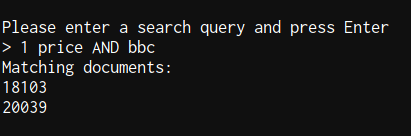
\includegraphics{conjunctive.png}
\end{figure}

\subsection{Phrase Query}

\begin{figure}[ht]
	\centering
	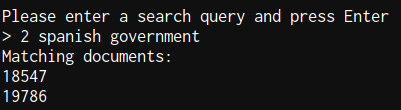
\includegraphics{phrase.png}
\end{figure}

\subsection{Proximity Query}

\begin{figure}[ht]
	\centering
	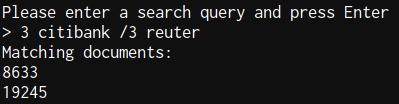
\includegraphics{proximity.png}
\end{figure}

\end{document}
